\label{sect:lsh_formulation}
Given a dataset $\mathbb{D}$ of size $n * d$, $n$ elements of $d$
features (or $n$ rows and $d$ columns), and a set $H(.)$ of $m$ hashing
functions, each element $x \in D$ is mapped to a binary vector of dimension
$m$ defined with $H(x)= [\; h_1(x),\;h_2(x), .., \;h_m(x)] $
\citep{chi_zhu_2017}

A hash function is said locality-sensitive if, for two points $x_i$ and $x_j$, it
satisfies the following conditions:
\begin{itemize}
    \item if $d(x_i, x_j) \leq R$ then $P(h(x_i )= h(x_j )) \geq p_1$.
    \item if $d(x_i,x_j) > cR$ then $P(h(x_i) = h(x_j)) <p_2$.
\end{itemize}
Where:
\begin{multicols}{2}
    \begin{itemize}
        \label{itemize:r-cR-equations}
        \item $c > 1 \in \mathbb{R}$
        \item $p_1$ is the probability for nearby points.
        \item $p_2$ is the probability of points being far apart.
    \end{itemize}
\end{multicols}

The gap between $p_1$ and $p_2$ is quantified by the parameter $c$, and it
determines how sensitive the hash function is to the changes in distance, the
formula of this sensitivity is given by: $\rho = \frac{\log{1/ p_1}}{\log{1/
            p_2}}$

The figure \ref{fig:r_cr_condition} below, shows in the red zone the meaning of
the first condition that consists of having all the points in the red circle
colliding with the query point with a high probability. While the second
condition is shown in the blue zone which means that all the points in the
purple circle have a small probability of colliding with the query point.

\begin{figure}[h]
    \centering
    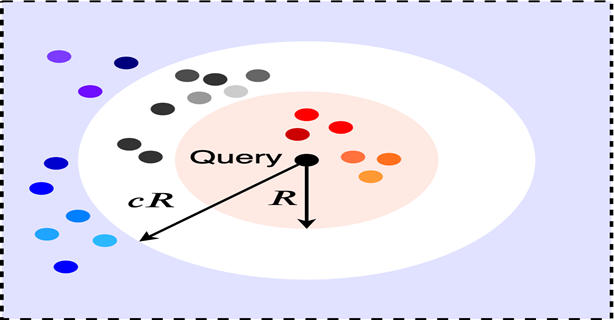
\includegraphics{state_of_the_art/r-cr conditions.png}
    \caption{Locality-Sensitive Hash Family demonstration. Source:
        \href{https://randorithms.com/2019/09/19/Visual-LSH.html}{Blog in
            randorithms}}
    \label{fig:r_cr_condition}
\end{figure}

The distance function $d$ mentioned in the two conditions
\ref{itemize:r-cR-equations} can be different depending on the nature of the
treated problem, and so are the hashing functions used in LSH which can estimate
different metrics.